\documentclass[american,aps,pra,reprint,floatfix,nofootinbib,superscriptaddress]{revtex4-2}
% General document formatting
\usepackage{tikz}
\usepackage[margin=0.7in]{geometry}
\usepackage{xintfrac}
\usepackage{braket}
% Documentation:
% https://ftp.cc.uoc.gr/mirrors/CTAN/macros/latex/contrib/parskip/parskip.pdf
\usepackage[utf8]{inputenc}

% Math packages:
\usepackage{amsmath,amssymb,amsfonts,amsthm}

% Our definitions:
\DeclareMathOperator{\smoothen}{smoothen}
\DeclareMathOperator{\mean}{mean}
\DeclareMathOperator{\Tr}{Tr}
\DeclareMathOperator{\atantwo}{atan2}
\DeclareMathOperator{\real}{Re}
\DeclareMathOperator{\imag}{Im}
%\DeclareMathOperator{\arg}{arg}
\newcommand{\abs}[1]{\left|#1\right|}
\newcommand{\norm}[1]{\left\|#1\right\|}
\newcommand{\absmt}{\abs{m_{T}'}}
\newtheorem{theorem}{Theorem}

% Draft comments
\usepackage{xcolor}
\newcommand{\VK}[1]{\textcolor{green}{[VK: #1]}}
\newcommand{\DL}[1]{\textcolor{blue}{[DL: #1]}}
\newcommand{\NE}[1]{\textcolor{magenta}{[NE: #1]}}

\begin{document}

\title{Machine learning Fisher Information Metric from bitstrings}
\author{First Last}
\email{email}
\affiliation{USC affiliation}

\date{\today}

\begin{abstract}
We present a machine-learning based method ``Bitstring-ChiFc'' which,
given a dataset corresponding to a family of distributions of bitstrings
parameterized by a manifold, can produce a rough approximation
for the corresponding Fisher Information Metric.
We observe that for multiple toy models there are often enough simple patterns
in the data that this approach
achieves satisfactory approximation even for dataset sizes small
compared to the number of possible bitstrings.
\end{abstract}

\maketitle

\section{Presentation}
\subsection{Challenge: finding phase transitions}
Let's talk about phase transitions.  Consider the Hamiltonian
on a $2 \times L$ lattice given by the following equations.
\begin{equation}
  \label{eq:Hladder.1}
  H(s,K,U) = (1-s) H_0 + s H_1,
\end{equation}
\begin{equation}
  \label{eq:Hladder.2}
  H_0 = -\sum_{i=0}^{L-1} (X_{T_i} + X_{B_i}),
\end{equation}
\begin{multline}
  \label{eq:Hladder.3}
  H_1 = \sum_{i=0}^{L-1} \biggl(K Z_{T_i} Z_{T_{i+1}} - K Z_{T_i} Z_{B_i}
    - K Z_{B_i} Z_{B_{i+1}} \\
  - K Z_{T_i} + \frac{U}{2} Z_{B_i}\biggr).
\end{multline}
Here qubits $T_L$ and $B_L$ are identified with $T_0$ and $B_0$ respectively.

It is called ``Frustrated Ladder Hamiltonian'' and is schematically represented
by the following diagram:
\begin{center}
  \pgfmathparse{\columnwidth/10.7cm}%
  \edef\tikzscale{\pgfmathresult}%
  \begin{tikzpicture}[scale=\tikzscale]
    \foreach \x in {0,...,9}{
      \draw (\x,0) circle (0.3) node (n0x\x){$T_{\x}$};
      \draw (\x,-1) circle (0.3) node (n1x\x){$B_{\x}$};
      \draw (n0x\x) -- (n1x\x);
    }
    \foreach \x[count=\xnext from 1] in {0,...,8}{
      \draw[dotted,line width=1pt] (n0x\x) -- (n0x\xnext);
      \draw (n1x\x) -- (n1x\xnext);
    }
    \draw[dotted,line width=1pt] (-0.7,0) -- (n0x0);
    \draw (-0.7,-1) -- (n1x0);
    \draw[dotted,line width=1pt] (9.7,0) -- (n0x9);
    \draw (9.7,-1) -- (n1x9);
  \end{tikzpicture}
\end{center}
On this diagram of $L=10$ Frustrated Ladder Hamiltonian
the solid lines represent ferromagnetic couplings and
dotted lines --- antiferromagnetic couplings. For a fixed $L$
the Frustrated Ladder Hamiltonian depends on 3 parameters, $s, K, U$.
We set $K=1$ and consider the values $s\in[0,1]$, $U\in[0,1]$.

How would one find phase transitions of that Hamiltonian? For that particular
Hamiltonian people already know a couple of order parameters given by the
following equations.
\begin{equation}
  \label{eq:mt}
  \absmt = \abs{\sum_i Z_{T_i}(-1)^i}
\end{equation}
\begin{equation}
  \label{eq:mb}
  m_B = \sum_i Z_{B_i}
\end{equation}

These are called ``staggered magnetization of the top row'' and ``magnetization
of the bottom row'' respectively. For $L=10$ we can compute these for various
values of the parameters of the Hamiltonian and produce the following diagrams:
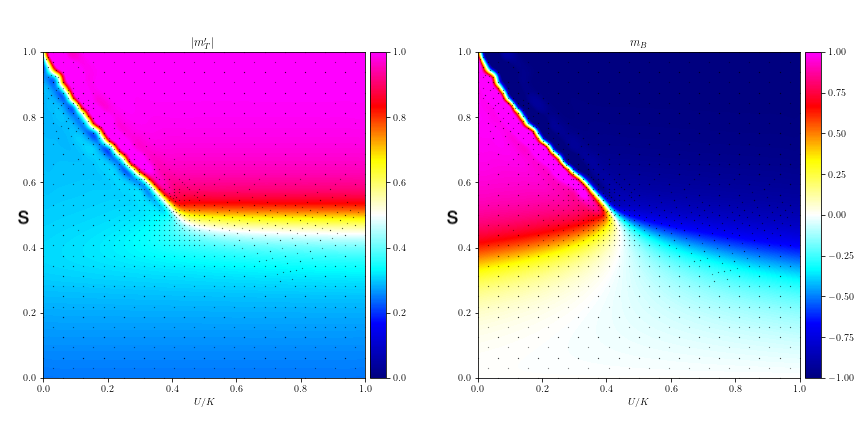
\includegraphics[width=\columnwidth]{lanczos_chi0_gp.png}

\VK{The following statement is in the direct contradiction with the statement
that the main goal of this paper is to learn Fisher Information Metric
given a dataset of bitstrings.}
In this work we focus on the task of identifying phase transitions in a
family of Hamiltonians $\{H_{\lambda}\}_{\lambda \in \Lambda}$ on a finite
set of qubits given an access to an oracle capable, given $\lambda \in \Lambda$,
of producing bitstrings measured in a computational basis from a state sampled
from a low temperature distribution corresponding to the Hamiltonian
$H_{\lambda}$. Specifically, the main goal of this paper is to make some
progress towards attempting to understand whether algorithms using
quantum computers can have an advantage over algorithms using the
same amount of resources but running on
purely classical hardware as illustrated on the following diagram.
\begin{center}
  \pgfmathparse{\columnwidth/13cm}%
  \edef\tikzscale{\pgfmathresult}%
  \begin{tikzpicture}[scale=\tikzscale]
    \newlength{\ux}
    \setlength{\ux}{15mm}
    \newlength{\uy}
    \setlength{\uy}{11mm}
    \draw (-3\ux, 0) node (H) {$\left\{H_\lambda\right\}$};
    \draw (0, 1.5\uy) node (A1)
      {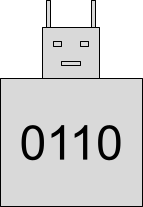
\includegraphics[width=0.15\columnwidth]{robot_classical.png}};
    \draw (0, -1.5\uy) node (A2)
      {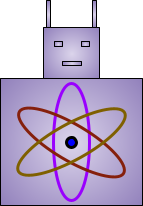
\includegraphics[width=0.15\columnwidth]{robot_quantum.png}};
    \draw (4\ux, 1.5\uy) node (B1)
      {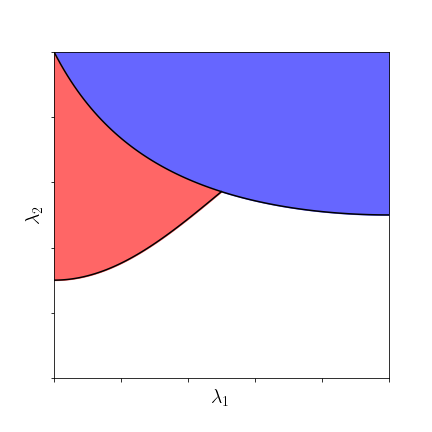
\includegraphics[width=0.28\columnwidth]{fake_phase_diagram.png}};
    \draw (4\ux, -1.5\uy) node (B2)
      {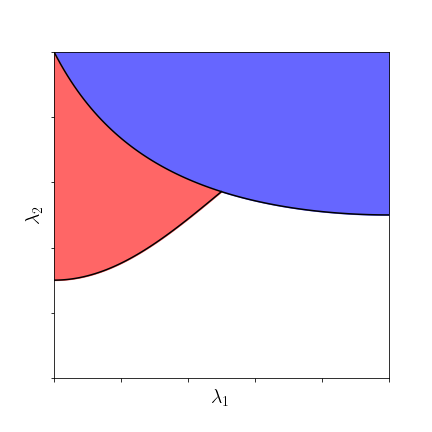
\includegraphics[width=0.28\columnwidth]{fake_phase_diagram.png}};
    \draw [->] (H.north) to[out=90,in=180] (A1.west);
    \draw [->] (H.south) to[out=-90,in=-180] (A2.west);
    \draw [->] (A1) -- (B1);
    \draw [->] (A2) -- (B2);
  \end{tikzpicture}
\end{center}
\VK{TODO: the idea of classical and quantum ``robots'' was taken from some
paper (probably Preskill). Find and cite that paper}

More specifically, throughout this work we consider algorithms attempting
to take an advantage of quantum computer having a specific structure. First,
we use quantum annealer to generate a dataset of bitstrings measured
in the computational basis corresponding
to various values of the parameters. Then we use a classical algorithm
involving machine learning
to process those bitstrings into an estimates of where phase transitions
are located. We also allow for an interactive version of this structure
where the classical part of the algorithm can produce additional requests
(values of the parameters and counts of samples requested) for the quantum
annealer generating bitstrings.
\begin{center}
  \pgfmathparse{\columnwidth/13cm}%
  \edef\tikzscale{\pgfmathresult}%
  \begin{tikzpicture}[scale=\tikzscale]
    \setlength{\ux}{15mm}
    \setlength{\uy}{11mm}
    \draw (-3\ux, 0) node (H) {$\left\{H_\lambda\right\}$};
    \draw (0, 1.5\uy) node (A1)
      {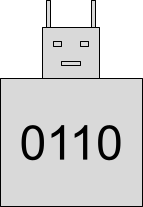
\includegraphics[width=0.15\columnwidth]{robot_classical.png}};
    \draw (-1.9\ux, -1.5\uy) node (A2a)
      {
\includegraphics[width=0.1\columnwidth]{qa.png}};
    \draw (-0.15\ux, -1.5\uy) node (A2b)
      {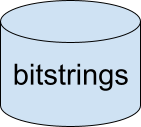
\includegraphics[width=0.15\columnwidth]{bitstrings.png}};
    \draw (1.6\ux, -1.5\uy) node (A2c)
      {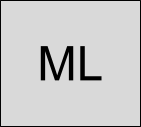
\includegraphics[width=0.1\columnwidth]{ml.png}};
    \draw (4\ux, 1.5\uy) node (B1)
      {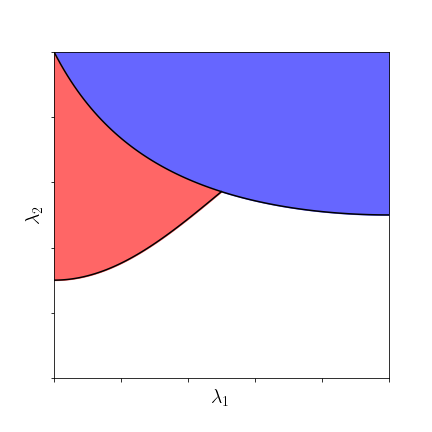
\includegraphics[width=0.28\columnwidth]{fake_phase_diagram.png}};
    \draw (4\ux, -1.5\uy) node (B2)
      {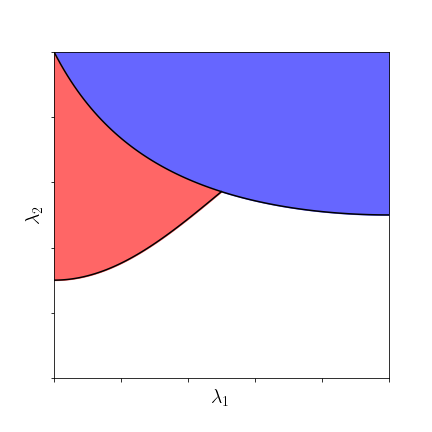
\includegraphics[width=0.28\columnwidth]{fake_phase_diagram.png}};
    \draw [->] (H.north) to[out=90,in=180] (A1.west);
    \draw [->] (H.south) to[out=-90,in=-180] (A2a.west);
    \draw [->] (A2a) -- (A2b);
    \draw [->] (A2b) -- (A2c);
    \draw [->] (A1) -- (B1);
    \draw [->] (A2c) -- (B2);
  \end{tikzpicture}
\end{center}

There could be other algorithms for this task taking an advantage of
quantum computers, but investigation of those is beyond the scope of this
paper.

There are 3 main challenges which need to be discussed before we can approach
specifying and solving this task.

\textbf{Issue 1: fixed finite size.}
One may observe, that we presented diagrams for fixed $L=10$ but wanted to
discuss phase transitions which are formally only defined in the thermodynamic
limit $L\to\infty$. That means, that one cannot see the actual phase transitions
on these diagrams, although one can see something which looks very close to
phase transitions: these are places where the color on these diagrams
changes quickly. Issue 1 is how to define the task of identifying
phase transitions for finite size Hamiltonians, where, strictly speaking,
there are no phase transitions due to finite fixed size.

\textbf{Issue 2: unknown order parameters.}
We want a method capable of identifying phase transitions in systems
for which these are not known yet. For those systems we may not know
what are the relevant order parameters. Issue 2 is how to define and
determine the phase transition in the absence of relevant known order parameters.

\textbf{Issue 3: loss of information at the time of measurement.}
ML algorithm only has access to bitstrings but, generally, bitstrings measured
in the computational basis do not contain
full information about the underlying quantum state.

There is a well-known approach \VK{TODO: cite} called fidelity susceptibility,
which we will use to address these issues. This is a quantity which
intuitively measures a squared rate of change of the underlying state.
By definition fidelity between two pure states $\ket{\phi}$ and $\ket{\psi}$ is
\begin{equation}
\label{eq:def.F.pure}
  F(\ket{\phi}, \ket{\psi}) = \abs{\braket{\phi\mid \psi}}.
\end{equation}
By definition fidelity between two mixed states
given by density matrices $\rho$ and $\sigma$ is
\begin{equation}
\label{eq:def.F.mixed}
  F(\rho, \sigma) = \Tr\left(\sqrt{\sqrt{\sigma}\rho\sqrt{\sigma}}\right).
\end{equation}
By definition classical fidelity between two discrete probability distributions
$p$ adn $q$
\begin{equation}
\label{eq:def.Fc}
  F_c(p, q) = \sum_z \sqrt{p_z q_z}.
\end{equation}
In this paper we apply classical fidelity mainly to distributions over bitstrings
$z$ obtained from measurement in the computational basis of some quantum states.

Fidelity susceptibility $\chi_F(s)$ is defined when there is a state $\rho(s)$
depending on some parameter $s$. In this case we write $F(s_1, s_2)$ instead
of $F(\rho(s_1), \rho(s_2))$. Then
term in the Taylor expansion of the fidelity:
\begin{equation}
\label{eq:def.chiF}
  F(s, s + \delta s) = 1 - \frac{\delta s^2}{2} \chi_F(s) + O(\delta s^3).
\end{equation}
Similarly, the classical fidelity susceptibility $\chi_{F_c}(s)$ is defined by
\begin{equation}
\label{eq:def.chiFc}
  F_c(s, s + \delta s) = 1 - \frac{\delta s^2}{2} \chi_{F_c}(s) + O(\delta s^3).
\end{equation}

Issues 1 and 2 are then solved by defining the task we are trying to solve
as the task of identifying the local maxima of fidelity susceptibility.
To address issue 3 we look at the properties of the fidelity
susceptibility, its classical counterpart, and relations between them.

\subsection{Motivation for the definition of the task}
Finite size systems in the sequence of systems experiencing a phase transition
in the thermodynamic limit are known to often experience maxima of fidelity susceptibility at or around the location of the phase transition. Intuitively, that
makes sense because the fidelity susceptibility measures the square rate of change of the underlying state and it is known that phase transitions correspond to rapid change of the underlying state.

\subsection{Properties of fidelity susceptibility}
Roughly speaking, we plan to prove the following properties.
\begin{itemize}
  \item Formula \eqref{eq:def.F.mixed} is consistent with \eqref{eq:def.F.pure}
    for pure states and with \eqref{eq:def.Fc} for probability distributions.
  \item Usually, for fidelity susceptibility (or classical fidelity
    susceptibility) to be defined, only one derivative of wave function
    (or probabilities) needs to exist.
  \item $0 \leq \chi_{F_c}(s) \leq \chi_F(s)$.
  \item $\mathbb{E}_{\textrm{measurements}} \chi_{F_c}(s) = \chi_F(s)/2$.
  \item For non-degenerate ground states of real-valued Hamiltonians
  $\chi_{F_c}(s) = \chi_F(s)$ almost everywhere.
\end{itemize}
See the below theorems for the exact statements.

\begin{theorem}
  \begin{enumerate}
    \item If $\ket{\phi}$ and $\ket{\psi}$ are pure states, then
      \begin{equation}
        F(\ket{\phi}, \ket{\psi}) =
          F(\ket{\phi}\bra{\phi}, \ket{\psi}\bra{\psi}).
      \end{equation}
    \item If $\rho$ and $\sigma$ are diagonal density matrices with diagonal entries
      equal to $\rho_{zz} = p_z$ and $\sigma_{zz} = q_z$ respectively, then
      \begin{equation}
        F(\rho, \sigma) = F(p, q).
      \end{equation}
    \item $F(\rho, sigma)$
  \end{enumerate}
\end{theorem}
\begin{proof}
  Suppose $\ket{\phi}$ and $\ket{\psi}$ are pure states. Then
  \begin{multline}
    F(\ket{\phi}\bra{\phi}, \ket{\psi}\bra{\psi}) \\ 
    = \Tr\left(
      \sqrt{\sqrt{\ket{\psi}\bra{\psi}}\ket{\phi}\bra{\phi}
      \sqrt{\ket{\psi}\bra{\psi}}}
    \right) \\
    = \Tr\left(
      \sqrt{\ket{\psi}\braket{\psi|\phi}\braket{\phi|\psi}\bra{\psi}}
    \right) \\
    = \abs{\braket{\psi|\phi}} \Tr\left(\ket{\psi}\bra{\psi}\right)
    = \abs{\braket{\psi|\phi}}
    = F(\ket{\phi}, \ket{\psi}).
  \end{multline}
  Suppose now $\rho$ and $\sigma$ are diagonal matrices with diagonal entries
  equal to $\rho_{zz} = p_z$ and $\sigma_{zz} = q_z$ respectively. Then
  \begin{multline}
    F(\rho, \sigma) = \Tr\left(\sqrt{\sqrt{\sigma}\rho\sqrt{\sigma}}\right) = \\
    \sum_z \sqrt{\sqrt{q_z} p_z \sqrt{q_z}} = \sum_z \sqrt{p_z q_z} = F(p, q).
  \end{multline}
  \VK{TODO:5: add part 2}
  \begin{multline}
    F(0, s) = F(\rho(0), \rho(s)) \\
    = \Tr\left(\sqrt{\sqrt{\sigma}\rho\sqrt{\sigma}}\right)
  \end{multline}
  \VK{TODO:5: add part 3}
\end{proof}

\begin{theorem}
\begin{enumerate}
  \item Suppose $\ket{\varphi(s)}$ is a state defined in the neighbourhood of
  $s = s_0 \in \mathbb{R}$ and differentiable at $s=s_0$.
  Then the fidelity susceptibility is well-defined at $s=s_0$ and is given by
  \begin{equation}
    \chi_F(s_0) = \norm{\dot\varphi_\perp(s_0)}^2,
  \end{equation}
  where $\varphi_\perp(s)$ is the component of $\ket{\varphi(s)}$ orthogonal
  to $\ket{\varphi(s_0)}$ and $\dot\bullet$ denotes the derivative with respect
  to $s$.
\end{enumerate}
\end{theorem}
\begin{proof}
Due to equivariance of the definitions with respect to translations of $s$,
without loss of generality we can prove the statements in the theorem for
$s_0 = 0$. Due to the absolute value in \eqref{eq:def.F.pure} we can multiply
$\ket{\varphi(s)}$ by $e^{-i\theta}$,
where $\theta = \arg(\braket{\varphi(0)|\varphi(s)})$,
without changing truthfullness of the conditions of the theorem
or the value of the fidelity susceptibility. Now we can express
\begin{equation}
\ket{\varphi(s)} = (1 - \alpha(s)) \ket{\varphi(0)} + \varphi_1(s),
\end{equation}
where $\alpha(s)$ is real and $\varphi_1(s)$ is orthogonal to $\varphi(0)$.
Also note that $\varphi_1(0) = 0$ and $\varphi_1(s)$ is differentiable at $s=0$.
\begin{multline}
  \label{eq:th1.eq1}
  F(0, s) = \braket{\varphi(0), \varphi(s)} = 1 - \alpha(s)
  = \sqrt{1 - \norm{\varphi_1(s)}^2}\\
  = 1 - \frac{s^2}{2} \norm{\dot\varphi_1(0)}^2 + o(s^2).
\end{multline}
Comparing \eqref{eq:th1.eq1} with \eqref{eq:def.chiF} we see that
$\chi_F(0)$ is defined and is equal to
\begin{equation}
  \chi_F(0) = \norm{\dot\varphi_\perp(0)}^2.
\end{equation}


\end{proof}

\begin{theorem}
Suppose a pure $s$-dependent state in a finite-dimensional Hilbert space
is described by a function
$(s_0 - \epsilon, s_0 + \epsilon) \to \mathcal{H}: s \mapsto \ket{\psi(s)}$,
which has a 1st derivative with respect to $s$ at $s=s_0$.
Then $\chi_F(s_0)$ is well-defined, $\chi_{F_c}$ is well-defined for any
orthogonal measurement basis, and
\begin{equation}
\mathbb{E}_{\textrm{measurements}} \chi_{F_c}(s_0) = \chi_F(s_0)/2,
\end{equation}
where the expectation $E_{\textrm{measurements}}$ is taken accross
all orthogonal bases in $\mathcal{H}$ using Haar measure (unique measure
invariant with respect to unitary rotations).
\VK{TODO: should ``measurements'' be italic in a formula inside a theorem?}
\end{theorem}
\begin{proof}
\VK{TODO:4}
\end{proof}

\begin{theorem}
Suppose there is a Hamiltonian $H(s)$ acting on a finite-dimensional Hilbert
space $\mathcal{H}$ with a basis $\{e_j\}_{j=1}^{d}$, which we will call
``computational basis''. \VK{TODO:5}
\begin{itemize}
  \item .
  \item a non-degenerage ground state $\ket{\psi(s)}$.
\end{itemize}
\end{theorem}
\begin{proof}
\VK{TODO:4}
\end{proof}

\subsection{Resolution of issue 3}
As we have seen in \VK{TODO: ref}, \VK{TODO: ref}, \VK{TODO: ref}
classical \VK{TODO}

\section{TODO}
\begin{enumerate}
\item Complete presentation section above.
\item Write down the proofs for the fidelity susceptibility claims below.
\item Describe the models and practical results for them.
\end{enumerate}

\section{Introduction}
TODO:

Such a family can arise, e.g., from measurements of a low-temperature
Gibbs ensemble of Hamiltonians parametrized by a parameter $\lambda$.

\section{Classical Fidelity Susceptibility}
Classical fidelity between 2 probability distributions $p$ and $q$ of
bitstrings $z$ is defined as
\begin{equation}
  F_c(p, q) = \sum_{z} \sqrt{p(z) q(z)}.
\end{equation}
We are interested in the fidelity between bitstring distributions at different
$s$ (e.g. $s=s_1$ and $s=s_2$), which we will denote as $F_c(s_1, s_2)$.

\NE{This is an example of a commonly used in-line comment which is separated by color. I could say something like: "This sentence is awkward" or "Needs citation" or very meta "Please use enquote for real quotes and not literal quotes."}

Fidelity susceptibility is defined as the term $\chi_{F_c}(s)$ in the Taylor
expansion
\begin{equation}
\label{eq:Fcs.Tailor}
  F_c(s, s+\delta s) = 1 - \frac{\delta s^2}{2} \chi_{F_c}(s) + O(\delta s^3).
\end{equation}
For such Taylor expansion to exist it is sufficient that the probabilities have
a Taylor expansion up to $O(\delta s^3)$. More generally, probability
distribution can depend on a point $\lambda$ on a manifold $\Lambda$,
in which case the Tailor expansion \eqref{eq:Fcs.Tailor} would become
\begin{equation}
\label{eq:Fcl.Tailor}
  F_c(\lambda, \lambda+\delta \lambda) = 1 - \frac{\delta \lambda_{j} \delta \lambda_k}{2} \chi_{F_c}^{jk}(\lambda) + O(\delta \lambda^3).
\end{equation}

\subsection{Classical and quantum fidelity susceptibility}
Fact 1: For pure states $\mathbb{E}\chi_{F_c} (s) = \frac12 \chi_F (s)$
where the expectation is over all orthogonal bases to perform the measurement in.

TODO:proof

Fact 2: For computational basis measurement of a non-degenerate ground state
of a real-valued Hamiltonian $H$, then $\chi_{F_c}(s) = \chi_F(s)$
almost everywhere.

TODO:proof

\section{Problem setup}
\begin{itemize}
  \item In this work we consider a family of distributions of
bitstrings $\{\mathcal{D}_{\lambda}\}_{\lambda \in \Lambda}$, each of length $n$.
  \item We are given a finite sample $\mathcal{D}_{\textrm{train}}$ of size $N$
  of pairs $(\lambda, z)$ s.t. $P(z|\lambda) = P_{\mathcal{D}_{\lambda}}(z)$.
  \item We are also given (possibly implicitly via coordinate description of $\Lambda$) a naive metric $g^0$ on $\Lambda$.
  \item We are asked to estimate the Fisher information metric $g$ on $\Lambda$ corresponding to distributions $\mathcal{D}_{\lambda}$.
  \item Locations with high $g / g^0$ are then considered to be conjectured locations of possible phase transitions.
\end{itemize}

We focus on the task of identifying phase transitions in that
family. Rigorously speaking, phase transitions are only defined
in the limit $n\to\infty$, while we are dealing with finite size systems.
A solution to that is to look at Fisher information metric: high distances according to Fisher information metric for points close according to naive metric likely correspond to phase transitions.

\section{Bitstring-ChiFc method}
In this work we propose the following method:
\begin{itemize}
  \item Collect training dataset $\mathcal{D}_{\chi_{F_c}\textrm{-train}}$ of
  the form $(\lambda_0, \delta \lambda, z, y)$, where $z$ is sampled from
  $p(\bullet, \lambda=\lambda_{z})$,
  $p_{+} = p(\lambda_{z} = \lambda_0 + \delta \lambda / 2| \lambda_{z} = \lambda_0 \pm \delta \lambda / 2)$, and
    $\mathbb{E}(y|\lambda_0, \delta \lambda, z) = p_{+}$.
    In practice $y \in \{0, 1\}$.
    Do it in the following way:
    \begin{itemize}
      \item Consider $\mathcal{D}_{\textrm{train}}$ consisting of pairs
      $(z, \lambda)$.
      \item Sample pairs $(z_{i{+}}, \lambda_{i{+}})$,
      $(z_{i{-}}, \lambda_{i{-}})$ from $\mathcal{D}_{\textrm{train}}$.
      \item Compute $\lambda_i = (\lambda_{i{+}} + \lambda_{i{-}})/2$,
      $\delta \lambda_i = \lambda_{i{+}} - \lambda_{i{-}}$.
      \item Add tuples $(\lambda_i, \delta \lambda_i, z_{i{+}}, 1)$ and $(\lambda_i, \delta \lambda_i, z_{i{-}}, 0)$ to the dataset $\mathcal{D}_{\chi_{F_c}\textrm{-train}}$.
    \end{itemize}
  \item Train a model $M$, which given $(\lambda_0, \delta \lambda, z)$
  will predict $l = M(\lambda_0, \delta \lambda, z)$
  s.t. $p_{+} = (1+e^{-l \cdot \delta \lambda})^{-1}$.
  Do this by minimizing cross-entropy loss on the dataset
  $\mathcal{D}_{\chi_{F_c}\textrm{-train}}$.
  \item Estimate
  \begin{multline}
  \chi_{F_c}^{jk}(\lambda) = \smoothen\Bigl(
  \lambda_1 \mapsto \mean_{(z, \lambda_1) \in \mathcal{D}_{\textrm{train}}}
  \bigl(\\
  M(\lambda_1, 0, z)_{j}M(\lambda_1, 0, z)_{k}\bigr)\Bigr)(\lambda).
  \end{multline}
\end{itemize}

\VK{TODO:2: expand the explanation for $s$ instead of $\lambda$.}

    \begin{multline*}
      \chi_{F_c}(\lambda) = \lim_{\delta \lambda\to 0} \frac2{\delta \lambda^2} \left(1 - \mathbb{E}_{z\sim Q(\bullet)} \frac{\sqrt{P(z|\lambda-\delta \lambda/2)P(z|\lambda+\delta \lambda/2)}}{Q(z)}\right)
      \\ \simeq \lim_{\delta \lambda\to 0} \mathbb{E}_{Q}\frac2{\delta \lambda^2}\frac{2\sinh^2(l\delta \lambda/4)}{\cosh(l\delta \lambda/2)} \simeq \frac14 \mathbb{E}_{z|\lambda} M(\lambda, 0, z)^2.
    \end{multline*}

TODO: models

TODO: experiments

\VK{TODO:2: 2nd part of the presentation with an image: presentation is a more low-low hanging fruit.}

\end{document}
